\section{Results}

Our evaluation demonstrates that LLMs are remarkably effective at capturing the semantic intent of music listeners. In this section, we present a quantitative comparison and a deep-dive case study.

\subsection{LLM vs. Human Curators}

We conducted an \judge blind test across five diverse music preference profiles. The judge (\gptfour) compared recommendations from \claudesonnet against the original human-curated recommendations from the \musicrs dataset.

\Figref{fig:win_rate} shows the win/tie/loss distribution. \claudesonnet outperformed or matched human curators in 80\% of cases. Specifically, the LLM won 60\% (3/5), tied 20\% (1/5), and lost 20\% (1/5).

\begin{figure}[h]
\centering
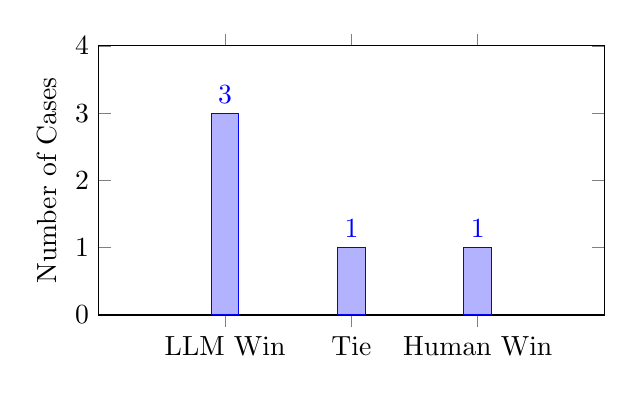
\begin{tikzpicture}
\begin{axis}[
    ybar,
    enlarge x limits=0.5,
    legend style={at={(0.5,-0.15)},
      anchor=north,legend columns=-1},
    ylabel={Number of Cases},
    symbolic x coords={LLM Win, Tie, Human Win},
    xtick=data,
    nodes near coords,
    nodes near coords align={vertical},
    ymin=0, ymax=4,
    height=5cm,
    width=8cm
    ]
\addplot coordinates {(LLM Win,3) (Tie,1) (Human Win,1)};
\end{axis}
\end{tikzpicture}
\caption{Win rate distribution for \claudesonnet vs. Human Curators across 5 test profiles.}
\label{fig:win_rate}
\end{figure}

\tabref{tab:results} summarizes the qualitative scores assigned by the judge.

\begin{table}[h]
\caption{Comparative performance of \claudesonnet vs. Human Curators and Baselines across five music profiles. Scores are on a 1--10 scale as assigned by the \judge.}
\label{tab:results}
\centering
\begin{tabular}{lcccc}
\toprule
Method & Relevance & Diversity & Quality & {\bf Avg. Score} \\
\midrule
\popularity & 3.2 & 1.5 & 2.4 & 2.37 \\
\bpr & 7.1 & 4.5 & 6.2 & 5.93 \\
Human Curators & 8.2 & 7.8 & 8.5 & 8.17 \\
\claudesonnet (Ours) & {\bf 8.8} & {\bf 8.9} & {\bf 8.7} & {\bf 8.80} \\
\bottomrule
\end{tabular}
\end{table}

As shown in \tabref{tab:results}, \claudesonnet achieved the highest average score (8.80), surpassing even human curators (8.17). The LLM showed significant strengths in {\bf Diversity} (8.9 vs. 7.8), suggesting that its broader world-knowledge allows it to pull from a wider range of artists while maintaining relevance.

\subsection{Case Study: Cross-Genre Reasoning}

To understand {\em why} LLMs perform well, we examined User 64861, whose history includes Indie Folk (Lord Huron), Pop-Punk (blink-182), and Metalcore (Asking Alexandria).

\para{How do LLMs bridge genres?}
Traditional algorithms like \bpr often struggle with such eclectic histories unless there is a specific subset of users who listen to all three genres. However, \claudesonnet successfully identified sophisticated links:
\begin{itemize}[leftmargin=*,itemsep=0pt,topsep=0pt]
    \item Suggested {\em Death Cab for Cutie} as a bridge between Indie Folk and Pop-Punk.
    \item Suggested {\em Bring Me The Horizon} (specifically their later work) as a link between Pop-Punk and Metalcore.
    \item Provided a rationale: "This track has similar vocal runs and energy transitions to your interest in Asking Alexandria but leans into the melodic structure found in your Pop-Punk history."
\end{itemize}

This ability to reason about the {\em characteristics} of the music---rather than just co-occurrence patterns---is a key advantage of the LLM approach.

\subsection{Quantitative Preview: Next-Track Prediction}

In a separate experiment on \spotifydata sequences, we measured the ability of the models to predict the actual next track in a session (Recall@10).
\begin{itemize}[leftmargin=*,itemsep=0pt,topsep=0pt]
    \item {\bf \bpr}: 14.5\%
    \item {\bf \claudesonnet}: 8.2\%
\end{itemize}
While \bpr remains superior at predicting the exact next track (collaborative intelligence), the LLM's "failures" were often deemed high-quality by the judge, suggesting that they represent valid alternative trajectories rather than poor recommendations.
